\chapter{Results}
\label{chap:Results}

\indent Unblinded signal region distributions of the kinematic variables with the most discrimination power are shown in figure \ref{fig:SRCUnblined}.  The expected background yield have been normalized to all control regions using the background only fitting procedure described in section \ref{sec:stat:bkgonly}.  \\

\begin{figure}[!hp] 
\begin{center}
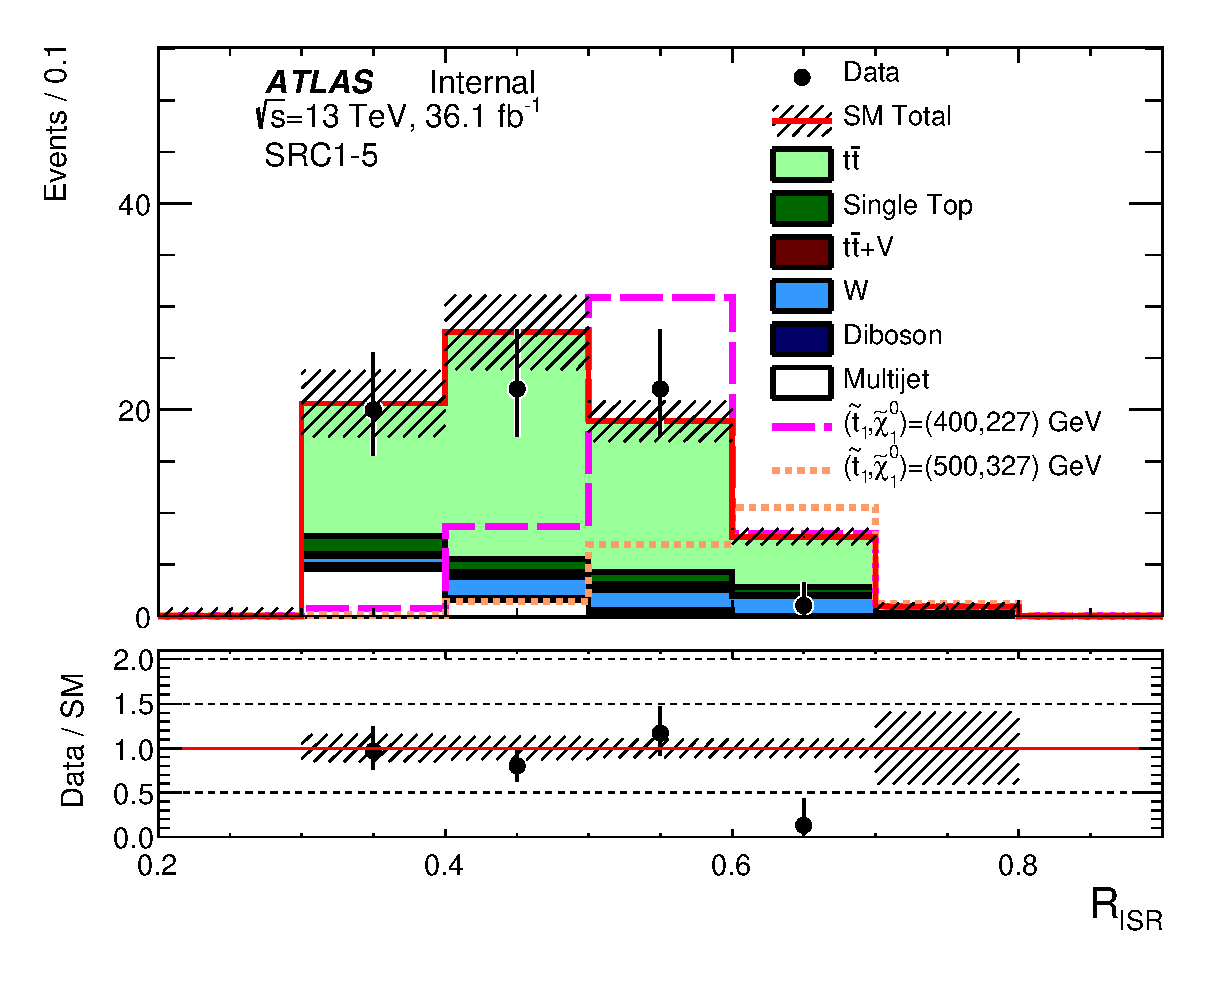
\includegraphics[width=0.85\textwidth]{figures/SRC/CA_RISR_SRC1_5}
%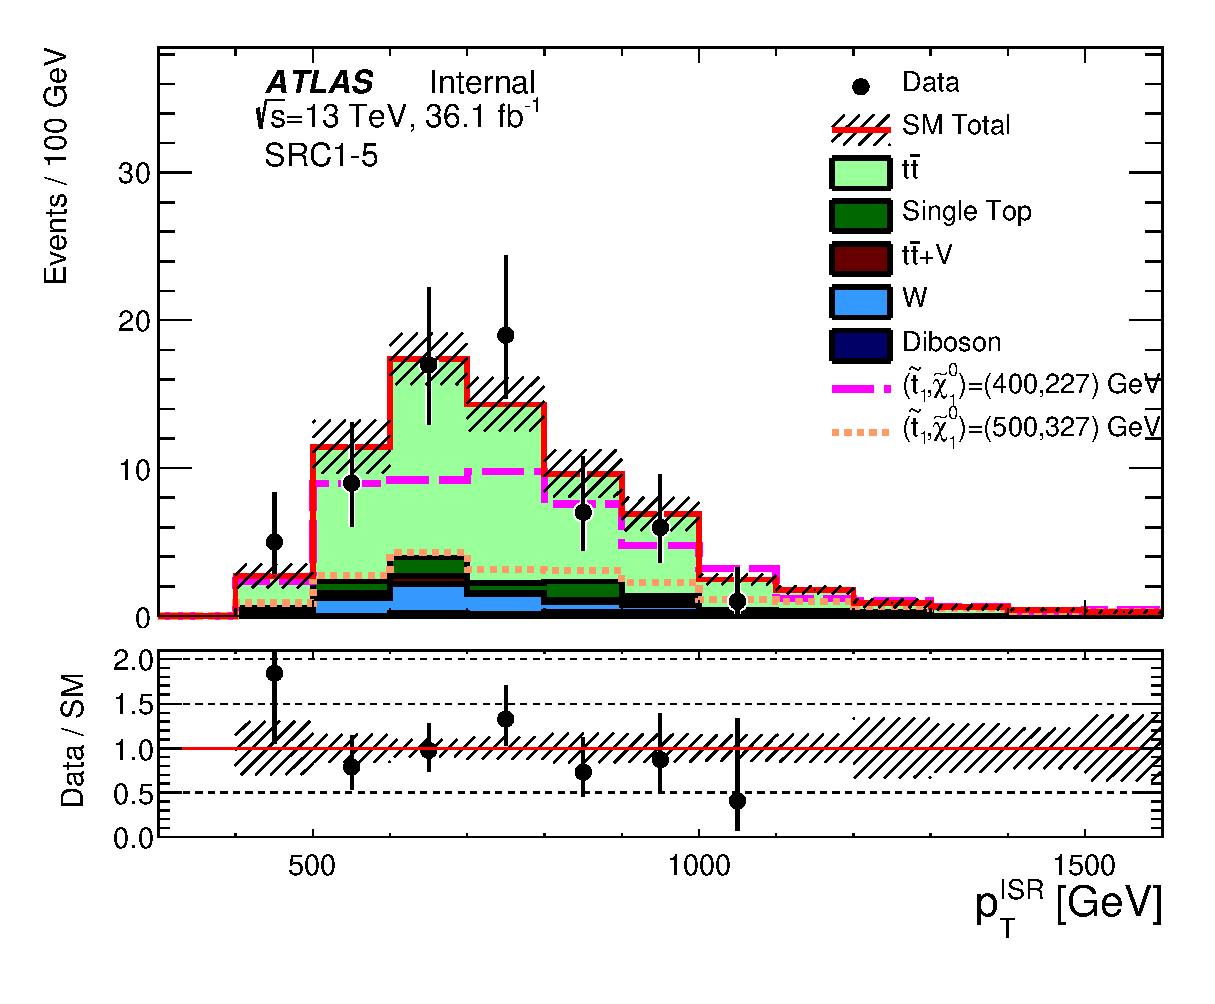
\includegraphics[width=0.45\textwidth]{figures/SRC/CA_PTISR_SRC1_5}
%\caption{Unblinded \rISR\ and \pTISR\ distributions for SRC1-5 for \intlumi\ \ifb.}
\caption{Unblinded $\rISR$  distributions for SRC1-5 for \intlumi\ \ifb.}
\label{fig:SRCUnblined}
\end{center}
\end{figure}

\indent Signal region yields with $\intlumi$ $\ifb$ of data can be seen in table \ref{table.bkgonly.SRC1to3} and \ref{table.bkgonly.SRC4to5}.  No significant excess is observed in any region.  An under fluctuation of background is observed in the $\RISR$ bin between $0.6-0.7$ but is not statistically significant due to the low amount of expected events.  \\



\begin{table}
\begin{center}
\setlength{\tabcolsep}{0.0pc}
{\small
%%
\begin{tabular*}{\textwidth}{@{\extracolsep{\fill}}lrrr}
\noalign{\smallskip}\hline\noalign{\smallskip}
{\bf SRC yields}           & SRC1            & SRC2            & SRC3              \\[-0.05cm]
\noalign{\smallskip}\hline\noalign{\smallskip}
%%
Observed events          & $23$              & $22$              & $23$                    \\
\noalign{\smallskip}\hline\noalign{\smallskip}
%%
Fitted bkg events         & $13.89 \pm 2.89$          & $25.32 \pm 4.29$          & $18.02 \pm 2.64$              \\
\noalign{\smallskip}\hline\noalign{\smallskip}
%%
        Fitted TTbar events         & $11.25 \pm 2.99$          & $21.39 \pm 3.67$          & $14.64 \pm 2.36$              \\
%%
        Fitted Wjets events         & $0.64 \pm 0.19$          & $1.59 \pm 0.44$          & $1.54 \pm 0.57$              \\
%%
        Fitted Zjets events         & $0.00 \pm 0.00$          & $0.00 \pm 0.00$          & $0.00 \pm 0.00$              \\
%%
        Fitted TtbarV events         & $0.16_{-0.16}^{+0.28}$          & $0.52 \pm 0.44$          & $0.49 \pm 0.31$              \\
%%
        Fitted SingleTop events         & $1.42 \pm 0.98$          & $1.57 \pm 1.04$          & $0.85 \pm 0.36$              \\
%%
        Fitted Diboson events         & $0.41 \pm 0.24$          & $0.24 \pm 0.05$          & $0.51 \pm 0.20$              \\
%%     
 \noalign{\smallskip}\hline\noalign{\smallskip}
%%
MC exp. SM events              & $18.96$          & $35.08$          & $24.66$              \\
\noalign{\smallskip}\hline\noalign{\smallskip}
%%
        MC exp. TTbar events         & $16.68$          & $31.72$          & $21.70$              \\
%%
        MC exp. Wjets events         & $0.57$          & $1.42$          & $1.37$              \\
%%
        MC exp. Zjets events         & $0.00$          & $0.00$          & $0.00$              \\
%%
        MC exp. TtbarV events         & $0.13$          & $0.41$          & $0.38$              \\
%%
        MC exp. SingleTop events         & $1.17$          & $1.29$          & $0.70$              \\
%%
        MC exp. Diboson events         & $0.41$          & $0.24$          & $0.51$              \\
%%     \\
\noalign{\smallskip}\hline\noalign{\smallskip}
\end{tabular*}
%%%
}
\end{center}
\caption{Region: SRC. Background-only fit results for an integrated luminosity of 36.47 \ifb. The uncertainties are statistical and systematic.
}
\label{table.bkgonly.SRC1to3}
\end{table}
%



\begin{table}
\begin{center}
\setlength{\tabcolsep}{0.0pc}
{\small
%%
\begin{tabular*}{\textwidth}{@{\extracolsep{\fill}}lrr}
\noalign{\smallskip}\hline\noalign{\smallskip}
{\bf SRC yields}           & SRC4            & SRC5              \\[-0.05cm]
\noalign{\smallskip}\hline\noalign{\smallskip}
%%
Observed events          & $1$              & $0$                    \\
\noalign{\smallskip}\hline\noalign{\smallskip}
%%
Expected bkg events         & $8.14 \pm 1.39$          & $0.99 \pm 0.71$              \\
\noalign{\smallskip}\hline\noalign{\smallskip}
%%
        Expected TTbar events         & $4.92 \pm 0.98$          & $0.63_{-0.63}^{+0.69}$              \\
%%
        Expected Wjets events         & $1.93 \pm 0.45$          & $0.21 \pm 0.12$              \\
%%
        Expected Zjets events         & 0.45 $\pm$ 0.24          & 0.09 $\pm$ 0.04             \\
%%
        Expected TtbarV events         & $0.08 \pm 0.08$          & $0.06 \pm 0.03$              \\
%%
        Expected SingleTop events         & $0.72_{-0.72}^{+0.77}$          & $0.00 \pm 0.00$              \\
%%
        Expected Diboson events         & $0.00 \pm 0.00$          & $0.00 \pm 0.00$              \\
%%
        Expected Multijets events         & $0.04 \pm 0.02$          & $0.00 \pm 0.00$              \\
%%     
 \noalign{\smallskip}\hline\noalign{\smallskip}
\end{tabular*}
%%%
}
\end{center}
\caption{Region: SRC. Background-only fit results for an integrated luminosity of 36.07 \ifb. The uncertainties are statistical and systematic.
}
\label{table.bkgonly.SRC4to5}
\end{table}
%


\indent 95 percent upper confidence limits on the observed cross-section ($\langle\epsilon\sigma\rangle_{\rm obs}^{95}$) and on the number of signal events ($S_{\rm obs}^{95}$) in each $\RISR$ bin is shown in table \ref{table.results.exclxsec.pval.upperlimit}.  Observed limits are derived using the discovery fit procedure described in section \ref{sec:stat:discovery}.  Discovery p-values are calculated using the asymptotic high statistics assumption.  \\


\begin{table}[!h]
\centering
\setlength{\tabcolsep}{0.0pc}
\begin{tabular*}{\textwidth}{@{\extracolsep{\fill}}lccccc}
\noalign{\smallskip}\hline\noalign{\smallskip}
{\bf Signal channel}                        & $\langle\epsilon{\rm \sigma}\rangle_{\rm obs}^{95}$[fb]  &  $S_{\rm obs}^{95}$  & $S_{\rm exp}^{95}$ & $CL_{B}$ & $p(s=0)$ ($Z$)  \\
\noalign{\smallskip}\hline\noalign{\smallskip}
%%
SRC1    & $0.44$ &  $16.0$ & $ { 16.3 }^{ +5.8 }_{ -4.2 }$ & $0.47$ &
 $ 0.50$~$(0.00)$ \\%
SRC2    & $0.35$ &  $12.6$ & $ { 15.5 }^{ +5.9 }_{ -4.2 }$ & $0.26$ &
$ 0.50$~$(0.00)$ \\%
SRC3    & $0.44$ &  $15.8$ & $ { 12.8 }^{ +4.7 }_{ -2.7 }$ & $0.69$ &
$ 0.30$~$(0.54)$ \\%
SRC4    & $0.09$ &  $3.1$ & $ { 6.5 }^{ +3.3 }_{ -2.1 }$ & $0.02$ & $
0.50$~$(0.00)$ \\%
SRC5    & $0.06$ &  $2.2$ & $ { 2.8 }^{ +2.0 }_{ -1.1 }$ & $0.32$ & $
0.49$~$(0.02)$ \\%

\noalign{\smallskip}\hline\noalign{\smallskip}
\end{tabular*}
\caption[Breakdown of upper limits.]{
Left to right: 95\% CL upper limits on the visible cross section
($\langle\epsilon\sigma\rangle_{\rm obs}^{95}$) and on the number of
signal events ($S_{\rm obs}^{95}$ ).  The third column
($S_{\rm exp}^{95}$) shows the 95\% CL upper limit on the number of
signal events, given the expected number (and $\pm 1\sigma$
excursions on the expectation) of background events.
The last two columns
indicate the $CL_B$ value, i.e. the confidence level observed for
the background-only hypothesis, and the discovery $p$-value ($p(s = 0)$). 
\label{table.results.exclxsec.pval.upperlimit}}
\end{table}
%
